\documentclass{article}

% Math packages
\usepackage{amsthm, amssymb, enumitem}

% Margins settings
\usepackage[margin=1.2in]{geometry}

% Bracket notation (quantum computing/information)
\usepackage{tikz}
\usetikzlibrary{quantikz}
\usepackage{braket}

% Spacing
\usepackage{parskip}
\usepackage{centernot}

% Required for inserting images
\usepackage{graphicx}
\graphicspath{{./Figures/}}

% Hyperlinks
\usepackage[colorlinks=true, allcolors=blue]{hyperref}

% Header
\usepackage{fancyhdr}
\pagestyle{fancy}
\lhead{November 6th, 2024}
\chead{Optimization for Data Science}
\rhead{University of Waterloo}

% Custom commands
\newcommand{\R}{\mathbb{R}}             % real numbers
\newcommand{\E}{\text{E}}               % expectation
\newcommand{\x}{\vec{x}}                % vector x
\newcommand{\y}{\vec{y}}                % vector y
\newcommand{\z}{\vec{z}}                % vector z
\newcommand{\dom}{\text{dom}}           % domain
\newcommand{\relint}{\text{relint}}     % relative interior
\newcommand{\ds}{\displaystyle}
\newcommand{\indep}{\perp\!\!\!\perp}

\newcommand{\rl}[1]{\left(#1\right)}

\setlength\parindent{0pt}

\title{CO 673/CS 794 - Optimization for Data Science\\Lecture 17 Notes}
\author{University of Waterloo}
\date{November 6th, 2024, 11h30-12h50 in MC 2054}

\begin{document}

\maketitle

\section{Administration}

\begin{itemize}
    \item Problem set 5 to be posted today, due Friday, November 15th, at 19h00
\end{itemize}

\section{Minimization of composite functions}

Recall from the previous lecture:

\textbf{Theorem.} Suppose that $f \colon \R^n \to \R$ is $L$-smooth, $m$-strongly convex, where $m > 0$. Suppose that $\psi \colon \R^n \to \R$ is closed, proper, and convex. Let $F = f + \psi$. Then, $F$ has a unique minimizer.

\begin{proof}
    Uniqueness follows from strict convexity.

    Existence:

    Let $\x_0 \in \relint(\dom(\psi))$. Let $S = \{x : F(\x) \leq F(\x_0)\}$.

    \textit{Claim:} $S$ is bounded.
    \begin{proof}
        Let $\vec{g} \in \partial \psi(\x_0)$. Previously, we showed that $S \subseteq \overline{B}_r(\x_0)$ where $r = \frac{2}{m}\|\vec{g} + \nabla f(\x_0)\|$.
    \end{proof}

    \textit{Claim:} $F$ is bounded above on $S$. This is obvious for the reason that $F(\x) \leq F(\x_0)$.

    \textit{Claim:} $F$ is bounded below on $S$.

    \begin{proof}
        $\forall \x \in S$, by the subgradient inequality,
        \begin{align*}
            F(\x) &\leq F(\x_0) + (\vec{g} + \nabla f(\x_0))^\top(\x - \x_0) \\
            &\leq F(\x_0) - \|\vec{g} + \nabla f(\x_0)\| \cdot \|\x - \x_0\| \tag{Cauchy-Schwartz inequality} \\
            &\leq F(\x_0) - \|\vec{g} + \nabla f(\x_0)\| \cdot \frac{2}{m}\|\vec{g} + \nabla f(\x_0)\| \tag{by the earlier claim}
        \end{align*}
        This proves the claim.
    \end{proof}

    Consider $Q =$ epi$F \cap \left(S \times \left[\inf\left(\{F(\x) : \x \in S\}\right);\; \sup\left(\{F(\x) : \x \in S\}\right)\right]\right)$.

    % IMAGE

    Both sets are closed, the second set is compact, thus $Q$ is compact. THis implies  that $\Phi \colon Q \to \R$, such that $\Phi(\x,\, \y)$ attains its minimizer, say $(\x^*,\, \y^*)$. Then, $\x^* \in S$, $(\x^*,\, \y^*) \in$ epi$F$, and $\y^* = F(\x^*)$. If instead $\y^* > F(\x^*)$, it would contradict the minimality with respect to $\Phi$.

    Thus, $\x^*$ must be a minimizer of $F$ over $S$.

    Additionally, $\forall \x \in \R^n \setminus S$, $F(\x^*) \leq F(\x)$, as $\forall \x \notin S$, $F(\x) \overset{(1)}{>} F(\x_0) \overset{(2)}{\geq} F(\x^*)$, where $(1)$ holds by definition of $S$, and $(2)$ hods because $\x_0 \in S$, over which $\x^*$ minimizes $S$.

    Therefore, $\x^*$ is a global minimizer fo $F$.
\end{proof}

Prox: Let $\psi \colon \R^n \to \R \cup \{\infty\}$ be proper, closed, and convex. Then,
\begin{align*}
    \text{prox}_{\psi}(\x) = \text{argmin}_{\z}\left(\left\{\psi(\z) + \frac{1}{2}\|\z - \z\|^2\right\}\right)
\end{align*}
where ``min'' outputs the minimum, and ``argmin'' outputs the minimizer.

\textbf{Theorem.} Let $\psi$ be defined as above. $\forall \x$, if $q(\z) := \psi(\z) + \frac{1}{2}\|\z - \x\|^2$, then $q$ has a unique minimizer.

This imolues that $\text{prox}_\psi$ is well-defined.

\begin{proof}
    Follows from the previous theorem as $z \mapsto \frac{1}{2}\|\z - \x\|^2$ is $1$-smooth, and $1$-strongly convex.
\end{proof}

We say that $\psi$ is ``proximable'' if there is an efficient procedure to evaluate $\text{prox}_\psi(\x)$.

Example 1. $f(x) = t|x|$ where $t > 0$.

Given $x \in R$,
\begin{align*}
    q(z) &= t|z| + \frac{1}{2}(z - x)^2 \\
    \partial q(z) &= t\partial |z| + z - x
\end{align*}

Fact 1: If $g \colon \R^n \to \R \cup \{\infty\}$ is convex, $\x \in \dom(g)$, then $\forall t > 0$, $\partial (tg)(\x) = t \partial g(\x)$.

Note: breaking up the sum is ok because C.Q. holds:
\[
    \underbrace{\relint(\dom(|\cdot|))}_{\R} \cap\, \relint\left(\underbrace{\dom\left(z \mapsto \frac{1}{2}(z - x)^2\right)}_{\R}\right) \neq \varnothing
\]

Fact:
\[
    \partial |x| = \begin{cases}
        \{-1\}, & x < 0 \\
        [-1;\; 1], & x = 0 \\
        \{1\}, & x > 0
    \end{cases}
\]

\begin{center}
    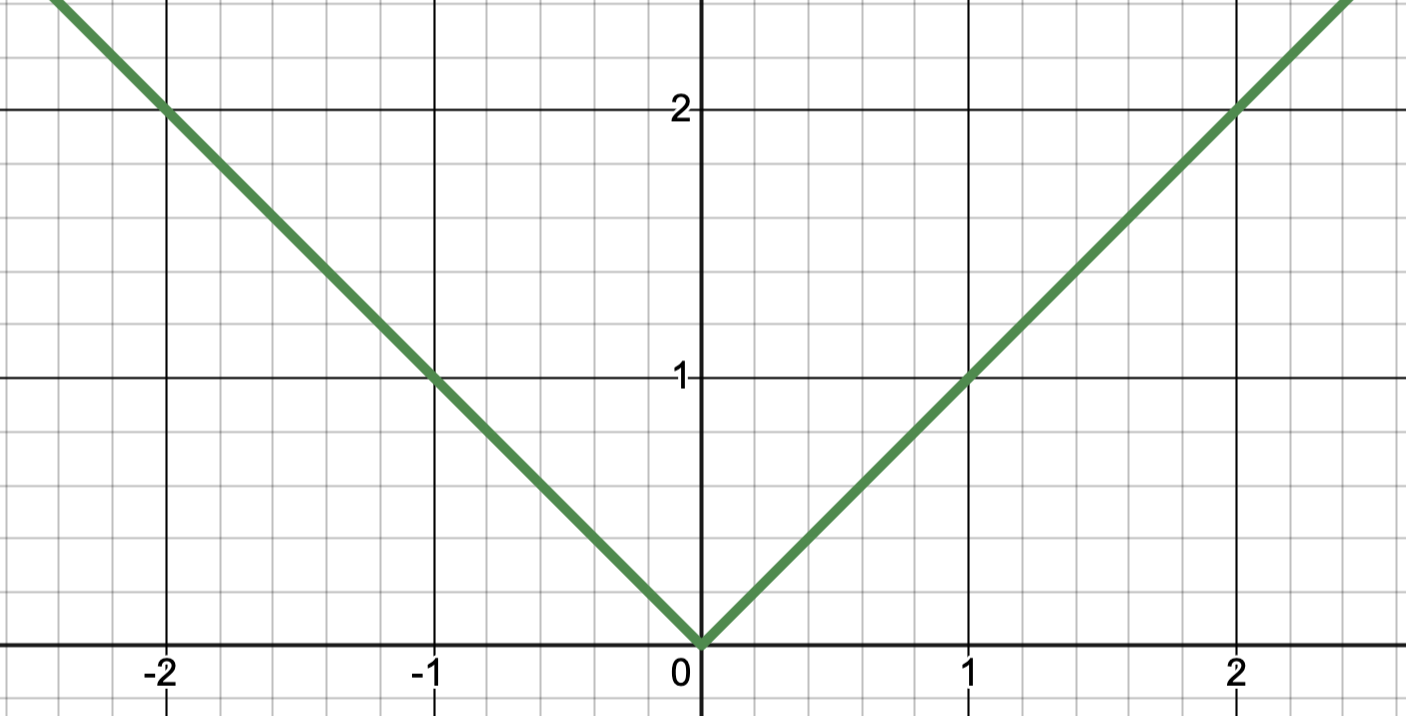
\includegraphics[scale=0.4]{abs_x.png}
\end{center}

Example 2:
$\implies$:
\[
    \partial q(z) = \begin{cases}
        \{-t + z - x\}, & z < 0 \quad \text{(a)} \\
        [-t + z - x;\; t + z - x], & z = 0 \quad \text{(b)} \\
        \{t + z - x\}, & x > 0 \quad \text{(c)}
    \end{cases}
\]
Must find $z$ such that $0 \in \partial q(z)$.

Case (a):
\begin{align*}
    0 = -t + z - x \iff z = x + t
\end{align*}
This is valid assuming $z < 0$, i.e., assuming $x + t < 0 \iff x < -t$.

Case (b):
\begin{align*}
    -t + z - x \leq 0 \leq t + z - x
\end{align*}
But $z = 0$, so
\begin{align*}
    -t - x \leq 0 \leq t - x
\end{align*}
i.e., $-t \leq x \leq t$

Case (c):
\begin{align*}
    0 = t + z - x \iff z = x - t
\end{align*}
This is valid assuming $z > 0$, i.e., $x > t$.

Summary:
\[
    \text{prox}_{t | \cdot |}(x) = \begin{cases}
        x + t, & x \leq -t \\
        0, & -t \leq x \leq t \\
        x - t, & x \geq t
    \end{cases}
\]

Extension to example 2:
\[
    \text{prox}_{t \|\cdot\|_1}(\x) = \vec{u}
\]
where
\[
    u_j = \begin{cases}
        x_j + t, & x_j < -t \\
        0, & x_j \in [-t;\; t] \\
        x_j - t, & x_j > t
    \end{cases}
\]
Note: $1$-norm is separable, meaning that it can be written as $f_1(x_1) + \ldots + f_n(x_n)$

Problem set 5: partly separable.

Example 3: $\text{prox}_{t \|\cdot\|}$
\[
    \varphi(\x) = \|\x\| \quad \implies \quad \partial \varphi(\x) = \begin{cases}
        \left\{\frac{\x}{\|\x\|}\right\}, & \x \neq \vec{0} \\
        \overline{B}_1\left(\vec{0}\right), & \x = \vec{0}
    \end{cases}
\]
\[
    \frac{\partial}{\partial x_j} \sqrt{\sum_{j = 1}^{j = n} x_j^2} = \frac{x_j}{\sqrt{\sum_{j = 1}^{j = n} x_j^2}} \quad \implies \quad \nabla \|\x\| = \frac{\x}{\|\x\|}
\]
To prove the $\x = \vec{0}$ case in Problem Set 5, use the Cauchy-Schwartz inequality to show that
\[
    \overline{B}_1\left(\vec{0}\right) \subseteq \partial f(\x)
\]
Then, select $\vec{g}$ such that $\|\vec{g}\| > 1$. We must find $\y$ that violates the subgradient inequality.
\[
    \R^n \setminus \overline{B}_1\left(\vec{0}\right) \subseteq \R^n \setminus f(\x)
\]

\[
    \text{prox}_{t \|\cdot\|}(\x) = \text{argmin}_{\z}
\]
where $q(\z) = t\|\z\| + \frac{1}{2}\|\z - \x\|^2$.
\begin{align*}
    \vec{0} \in q(\z) \overset{\text{C.Q.}}{\iff} \vec{0} \in t\partial \|\cdot\|(\z) + \{\z - \x\} \\
    \iff \quad \x - \z \in \begin{cases}
        \overline{B}_t\left(\vec{0}\right), & \z = \vec{0}\, \text{(a)} \\
        \left\{\frac{t\z}{\|\z\|}\right\}, & \z \neq \vec{0}\, \text{(b)}
    \end{cases}
\end{align*}
Case (b):
\[
    \x - \z = \frac{t\z}{\|\z\|}
\]
must hold: $z$ a multiple of $\x$. Say $\z = \theta\x$:
\[
    \x - \theta\x = \frac{t\theta\x}{|\theta| \cdot \|\x\|}
\]
which requires $\theta > 0$. We ``divide both sides by $\x$'':
\[
    1 - \theta = \frac{t}{\|\x\|} \quad \implies \quad \theta = 1 - \frac{t}{\|\x\|}
\]
We observe that assuming $\|x\| > t$, then it is ok to ``divide by $\x$'' as $\x \neq \vec{0}$. So, in this case,
\[
    \z = \left(1 - \frac{t}{\|\x\|}\right)\x
\]

Case (a):

$\x - \z \in \overline{B}_t\left(\vec{0}\right)$ but $\z = \vec{0}$, so we have that $\x \in \overline{B}_t\left(\vec{0}\right)$.

We conclude that
\[
    \text{prox}_{t \|\cdot\|}(\x) = \begin{cases}
        \vec{0}, & \|\x\| \leq t \\
        \left(1 - \frac{t}{\|\x\|}\right)\x, & \|\x\| \geq t
    \end{cases}
\]
Given $f \colon \R^n \to \R$ is convex and $L$-smooth, $\psi \colon \R^n \to \R \cup \{\infty\}$ is proper, closed, convex, and proximable, and $F = f + \psi$.

Proximal gradient of $F$ at $\x$:
\[
    G_L(\x) = L\left(\x - \text{prox}_{\psi/L}\left(\x - \frac{1}{L}\nabla f(\x)\right)\right)
\]
We observe that if $\psi \equiv 0$, then,
\[
    \text{prox}_0(\x) = \text{argmin}_{\z}\left(\left\{0 + \frac{1}{2}\|\x - \z\|^2\right\}\right) = \x
\]
So,
\[
    G_L(\x) = L\left(\x - \x + \frac{1}{L}\nabla f(\x)\right) = \nabla f(\x)
\]
\textbf{Theorem.} (Proposition 9.3)
Define $F$ as above. Then, $G_L(\x) = \vec{0} \iff \x$ minimizes $F$.

\begin{proof}
    \begin{align*}
        G_L(\x) = \vec{0} &\iff \x - \text{prox}_{\psi/L}\left(\x - \frac{1}{L}\nabla f(\x)\right) = 0 \\
        &\iff \x = \text{prox}_{\psi/L}\left(\x - \frac{1}{L}\nabla f(\x)\right) \\
        &=\iff \x = \text{argmin}_{\z}\left(\left\{\frac{\psi(\z)}{L} + \frac{1}{2}\left\|\z - \x + \frac{1}{L}\right\|\right\}\right) \intertext{Take derivative with respect to $\vec{z}$, check C.Q.!}
        &\iff \vec{0} \in \left.\left[\frac{\partial \psi(\vec{z})}{L} + \vec{z} - \x + \frac{1}{L}\nabla f(\x)\right]\right|_{\vec{z} = \x} \\
        &\iff \vec{0} \in \frac{\partial \psi(\x)}{L} + \x - \x + \frac{1}{L}\nabla f(\x) \\
        &\iff \vec{0} \in \frac{1}{L} \rl{\partial \psi(\x) + \nabla f(\x)} \\
        &\iff \vec{0} \in \partial F(\x)
    \end{align*}
\end{proof}

\section{Proximal gradient descent}
\begin{verbatim}
x_0 in dom(psi) arbitrary
for k = 0, 1, 2, ...
    x_{k + 1} := x_k - (1/L)G_L(x)
\end{verbatim}

Accelerated proximal gradient descent (= FISTA Nesterov $\sim$ 2004, Beck + Teboulle $\sim$ 2013)

From AGD algorithm, replace
\[
    \x_{k + 1} := \y_k - \frac{1}{L} \nabla f(\y_k)
\]
with
\[
    \x_{k + 1} := \y_k - \frac{1}{L}G_L(\y_k)
\]
when to terminate PGD/APGD? Use:
\[
    \|G_L(\x)\| \leq \text{tol}
\]
Note: we cannot terminate using $\partial F$, as $F$ may not necessarily be differentiable. Ex. $F(x) = |x|$.

Note:
\begin{align*}
    \x_{k + 1} &= \y_k - \frac{1}{L}G_L(\x) \\
    &= \y_k - \frac{1}{L}L\rl{\y_k - \text{prox}_{\psi/L}\rl{\y_k - \frac{\nabla f(\z_k)}{L}}} \\
    &= \text{prox}_{\psi/L}\rl{\y_k - \frac{\nabla f(\z_k)}{L}}
\end{align*}

\textbf{Theorem.} For $F$ defined as above, assume that $F$ has a minizer $\x^*$. For proximal gradient descent, $F(\x_k) - F(\x^*) \leq \frac{L\|\x_0 - \x^*\|^2}{2k}$. The same result as gradient descent.

If $f$ is $m$-strongly convex for $m > 0$, then
\[
    \|\x_k - \x^*\| \leq \rl{\frac{L - m}{L + m}}^k \|\x_0 - \x^*\|
\]
For accelerated proximal gradient descent, $k^2$ in the denominator of the first formula, and $\rl{\frac{\sqrt{L} - \sqrt{m}}{\sqrt{L} + \sqrt{m}}}^k$ in the second formula.

\end{document}
